\subsection{Comparison with published sign-domain methods}
\label{sec:eval-compare}

\textbf{Material.} Besides the eight CIF sequences we use 19 native high-resolution, camera-captured Xiph sequences~\cite{xiph_media} (twelve at $1920\times1080$: crowd\_run, ducks\_take\_off, in\_to\_tree, old\_town\_cross, park\_joy, pedestrian\_area, riverbed, rush\_hour, station2, sunflower, tractor, blue\_sky; seven at $1280\times720$: mobcal, parkrun, shields, stockholm and the three \emph{vidyo} conferencing clips), 60 frames each. All covers are encoded with x264 \emph{medium} (Intra4$\times$4 and Intra16$\times$16, deblocking on), Constrained Baseline, QP 18, 22, 28 and 34, with GOP~1 (all intra) and GOP~30 (one IDR followed by P frames, so that drift into predicted frames is included).

\textbf{Methods.} All methods use the same channel and are fed random message bits: per IDR they place $N$ bits, $N=64$ (the system default) or $N=5\%$ of the IDR's candidates. Besides our two policies we re-implement the selection and mapping rules of four published trailing-one methods inside a sign-only channel: Kim \emph{et al.}~\cite{kim2007t1} (first trailing-one sign of luma blocks in decoding order), Lin \emph{et al.}~\cite{lin2012cavlc} (keyed luma blocks, XOR of all trailing-one signs), Wang and Ma~\cite{wang2018cavlc} (one host per $E$ candidates, $(1,3,2)$ matrix code; the paper fixes $E\in[12,20]$; we choose $E$ from the expected bits per host so that the hosts span the whole picture at the given payload), and a Liao-style per-macroblock trailing-one parity~\cite{liao2009t1,liao2012t1journal} (the original grouping is not fully specified in the sources we could access). Ma \emph{et al.}~\cite{ma2010drift} modify coefficient pairs and need neighbouring prediction modes, so it is not reducible to sign flips and is not included; codeword-substitution methods~\cite{mobasseri2007} are not reducible either. Because only the selection and mapping rules carry over, our numbers are not comparable with those reported in the original papers. Unit tests check that every method embeds exactly the message bits it claims.

\begin{table*}[t]
\centering
\caption{Embedding quality of the compared methods at 64 bits per IDR: median over sequences of PSNR-Y over all frames [dB] (x264 medium). GOP 30 includes the drift into 29 P frames per IDR.}
\label{tab:quality-compare}
\begin{tabular}{@{}lcccccccc@{}}
\toprule
& \multicolumn{4}{c}{CIF (8 sequences)} & \multicolumn{4}{c}{native 720p/1080p (19 sequences)} \\
\cmidrule(lr){2-5}\cmidrule(lr){6-9}
& \multicolumn{2}{c}{GOP 1} & \multicolumn{2}{c}{GOP 30} & \multicolumn{2}{c}{GOP 1} & \multicolumn{2}{c}{GOP 30} \\
Method & QP 22 & QP 34 & QP 22 & QP 34 & QP 22 & QP 34 & QP 22 & QP 34 \\
\midrule
\csname @@input\endcsname tables/quality.tex 
\bottomrule
\end{tabular}
\end{table*}

\begin{figure*}[t]
\centering
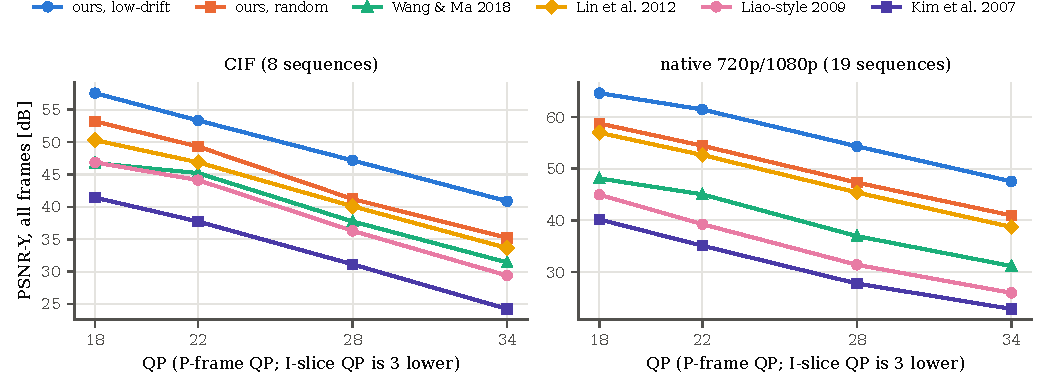
\includegraphics[width=\textwidth]{figures/quality_qp.pdf}
\caption{PSNR-Y (all frames, median over sequences) against QP at 64 bits per IDR, all-intra.}
\label{fig:quality-qp}
\end{figure*}

\textbf{Quality.} Table~\ref{tab:quality-compare} and Fig.~\ref{fig:quality-qp} show the same ordering at every QP, GOP and resolution. The low-drift policy is best: over the 16 settings (4 QPs, 2 GOPs, 2 rates) it gains 3.3--7.2\,dB over the uniform keyed choice on CIF (median 4.9\,dB; e.g.\ 53.3 vs.\ 49.3\,dB at QP~22 and 40.9 vs.\ 35.2\,dB at QP~34, all intra) and 3.3--8.0\,dB on native high resolution (median 5.9\,dB; 61.5 vs.\ 54.4\,dB at QP~22), and 3.9--9.2\,dB over the best baseline of each setting. The uniform keyed choice is in turn better than every baseline, because spreading carriers over the picture avoids the long intra-prediction chains that start at the top of the frame; the methods that fill blocks in decoding order are worst (Kim \emph{et al.}: 37.7\,dB at QP~22, 24.2\,dB at QP~34 on CIF). Parity and matrix codes change fewer signs per bit (Wang and Ma: 0.44 changes per bit against 0.50) but do not compensate for where they write: these methods use luma blocks only, whose sign changes propagate furthest with Intra4$\times$4 prediction (mean single-flip gain 35 for luma against 4 for chroma AC under this preset, Table~\ref{tab:single}), and parity and matrix codes may flip a lower-frequency trailing one than the first. No method changes the bit rate; the file size changed by one byte in a single run (an emulation-prevention byte).

\subsection{Steganalysis}
\label{sec:eval-steg}

\textbf{Protocol.} Covers are x264 medium, QP~22, all-intra encodes (CIF: 60 frames; high resolution: 10 frames, since feature extraction at 1080p is the bottleneck). Each of the six methods embeds at three rates: 64 bits per IDR, 5\% and 20\% of the IDR's candidates, giving 486 cover/stego pairs. The 27 sources are split by sequence into 17 for training, 3 for validation and 7 for testing (2 CIF and 5 high-resolution sequences, 160 frames per class), so no content is shared between training and testing. We use four detectors: (i)~323 compressed-domain features of the trailing-one signs (sign shares per category and coefficient class, joint sign patterns of a block, co-occurrences with the next level and with neighbouring blocks); (ii)~SPAM-686~\cite{pevny2010spam}; (iii)~a 3{,}978-dimensional reduced rich model (``SRM-lite'') following~\cite{fridrich2012srm}; features (i)--(iii) are classified with the FLD ensemble~\cite{kodovsky2012ensemble}; and (iv)~a Xu-Net-style CNN~\cite{xu2016xunet} trained on $256\times256$ luma tiles with early stopping on the validation sources. We report the minimum average error $P_E=\min(P_{\mathrm{FA}}+P_{\mathrm{MD}})/2$ on the test frames, the minimum taken over all thresholds of the test ROC as is customary~\cite{kodovsky2012ensemble}; this favours the detector (it is not a threshold fixed in advance), so it is conservative for claims of undetectability. With 320 test frames its standard error is about 0.03, so differences below 0.05 are not significant.

\begin{table*}[t]
\centering
\caption{Detection error $P_E$ on the test sources (0.5 = random guessing) per detector and embedding rate: 64 bits per IDR (system default), 5\% and 20\% of the IDR's candidates.}
\label{tab:steganalysis}
\setlength{\tabcolsep}{4pt}
\begin{tabular}{@{}lcccccccccccc@{}}
\toprule
& \multicolumn{3}{c}{CAVLC features} & \multicolumn{3}{c}{SPAM-686} & \multicolumn{3}{c}{SRM-lite} & \multicolumn{3}{c}{CNN} \\
\cmidrule(lr){2-4}\cmidrule(lr){5-7}\cmidrule(lr){8-10}\cmidrule(lr){11-13}
Method & 64 & 5\% & 20\% & 64 & 5\% & 20\% & 64 & 5\% & 20\% & 64 & 5\% & 20\% \\
\midrule
\csname @@input\endcsname tables/steganalysis.tex 
\bottomrule
\end{tabular}
\end{table*}

\begin{figure*}[t]
\centering
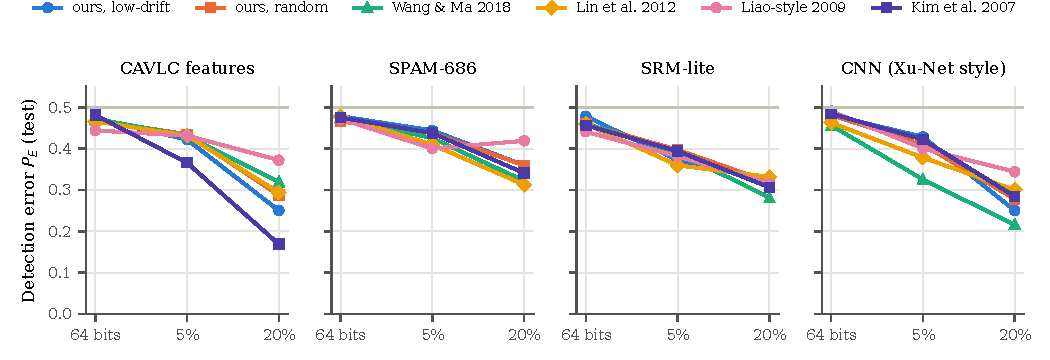
\includegraphics[width=\textwidth]{figures/steganalysis.pdf}
\caption{Detection error $P_E$ against the embedding rate for the four detectors.}
\label{fig:steganalysis}
\end{figure*}

\textbf{Results.} At the system's operating point of 64 bits per IDR no detector does better than guessing for any method ($P_E$ 0.44--0.49; AUC 0.50--0.55): about 32 sign changes among thousands of candidates per frame leave no measurable trace for these detectors. At 5\% of the candidates $P_E$ falls to 0.33--0.44 and at 20\% to 0.17--0.42 (Table~\ref{tab:steganalysis}, Fig.~\ref{fig:steganalysis}). The compressed-domain features are the strongest detector of the method that fills luma blocks in decoding order (Kim \emph{et al.}: $P_E=0.17$ at 20\%), whose changes concentrate in one region and one category. The low-drift policy is not easier to detect than the uniform keyed choice with the pixel-domain detectors (SPAM 0.36 vs.\ 0.36, SRM-lite 0.33 vs.\ 0.32) and slightly easier with the CAVLC features and the CNN at 20\% (0.25 vs.\ 0.29 and 0.25 vs.\ 0.28), differences within about one and a half standard errors. Concentrating carriers in cheap regions therefore buys 3--8\,dB of quality without a measurable loss of security at the rates the system uses; at high rates a small loss cannot be excluded.

These detectors are a lower bound on what a determined warden can do: the training set has 17 sequences, and stronger models (the full 34{,}671-dimensional SRM, SRNet-class networks, detectors that exploit the drift pattern of trailing-one changes~\cite{you2017cavlc}) and larger training sets may detect lower rates. We therefore claim covertness only at the default rate and only against the detectors tested.

\subsection{Native low-drift policy and verification tokens}
\label{sec:eval-native}
Table~\ref{tab:channel} runs the deployed native codec with a 201-byte payload (68-byte message and proof) at 64 bits per IDR on the 8 CIF and 19 native high-resolution covers (x264 medium, QP~22, all intra, 60 frames) for the four parameter combinations. In all 108 runs the master key extracts the exact payload and the stego file has the size of the cover. The low-drift policy raises the median PSNR-Y of the carrying frames by 3.9\,dB on CIF and 6.6\,dB on high resolution (61.1 vs.\ 54.5\,dB), and the worst frame by 6.4 and 10.8\,dB, at the same embedding time. In per-video key mode the token of each video extracts the payload and yields the same video digest as the master key in all 27 videos; the token of one video fails the frame check (``version is invalid'') on the next video in all 25 pairs tested; computing a token takes 0.07\,s at CIF and 0.7\,s at 1080p (one parse of the first IDR). Per-video keys add no measurable cost to embedding.

\begin{table}[t]
\centering
\caption{Native codec with both channel parameters (8 CIF and 19 native HD covers, 60 frames, 201-byte payload, 64 bits per IDR): runs, extraction with the key and with the token, PSNR-Y of carrying frames (median, minimum) and embedding time [s].}
\label{tab:channel}
\setlength{\tabcolsep}{3pt}
\footnotesize
\begin{tabular}{@{}lllrcccc r@{}}
\toprule
 & Select & Key mode & $n$ & key & token & PSNR & min & time \\
\midrule
\csname @@input\endcsname tables/channel.tex 
\bottomrule
\end{tabular}
\end{table}
